\section{SPY Visualize Sparsity Pattern of a Sparse Matrix}

\subsection{Usage}

Plots the sparsity pattern of a sparse matrix.  The syntax for its use is
\begin{verbatim}
   spy(x)
\end{verbatim}
which uses a default color and symbol.  Alternately, you can use
\begin{verbatim}
   spy(x,colspec)
\end{verbatim}
where \verb|colspec| is any valid color and symbol spec accepted by \verb|plot|.
\subsection{Example}

First, an example of a random sparse matrix.
\begin{verbatim}
--> y = sprand(1000,1000,.001);
Warning: Newly defined variable i shadows a function of the same name.  Use clear i to recover access to the function
Warning: Newly defined variable j shadows a function of the same name.  Use clear j to recover access to the function
--> spy(y,'ro')
Warning: Newly defined variable i shadows a function of the same name.  Use clear i to recover access to the function
Warning: Newly defined variable j shadows a function of the same name.  Use clear j to recover access to the function
\end{verbatim}
which is shown here


\centerline{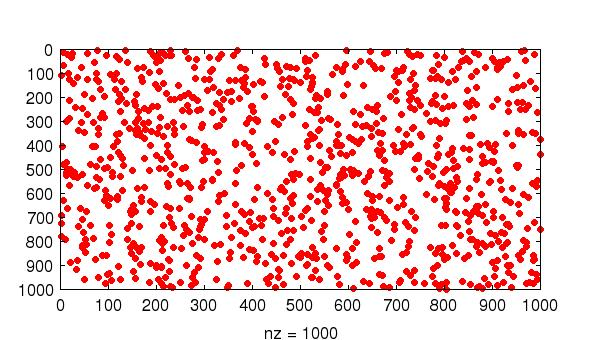
\includegraphics[width=8cm]{spy1}}

Here is a sparse matrix with a little more structure.  First we build a 
sparse matrix with block diagonal structure, and then use \verb|spy| to 
visualize the structure.
\begin{verbatim}
--> A = sparse(1000,1000);
--> for i=1:25; A((1:40) + 40*(i-1),(1:40) + 40*(i-1)) = 1; end;
--> spy(A,'gx')
Warning: Newly defined variable i shadows a function of the same name.  Use clear i to recover access to the function
Warning: Newly defined variable j shadows a function of the same name.  Use clear j to recover access to the function
\end{verbatim}
with the result shown here


\centerline{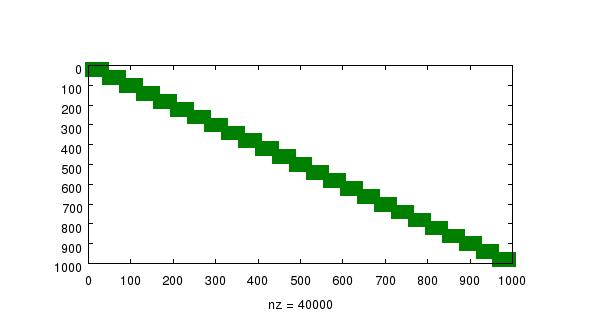
\includegraphics[width=8cm]{spy2}}

